\section{RQ1:  User-Level Factors in Toxicity on Twitter\label{sec:toxic_middle}}
Having provided background on our methodology and dataset, in this section, we discuss several of the user-level factors that coincide with and contribute to the toxicity on Twitter. 


\subsection{Setup}
Here, we examine the role of several user-level factors in contributing to or affecting the rate at which individual users are toxic on Twitter. Specifically, we examine the following user characteristics in contributing to or mitigating the toxicity of individual users on Twitter: 

\begin{enumerate}

\item \emph{The verified status of the account}
\item \emph{The number of years the account has been active on Twitter}
\item \emph{The log of the number of the account's followers}
\item \emph{The log of the number of accounts the user follows}
\item \emph{The account's partisanship as determined by our Correspondence Analysis}
\item \emph{The estimated average toxicity of all users the account mentioned/@ed on Twitter (\textit{i.e.}, accounts that the user has interacted with)}
\item  \emph{The estimated average partisanship of the accounts the user mentioned/@ed}
\item \emph{The standard deviation of the partisanship of the accounts that the user mentioned (\textit{i.e.}, the range of political views with which the user interacts)}
\item \emph{The average value of the partisanship of all accounts the user mentioned/@ed}
\item \emph{The average difference in the partisanship of the account the given user mentioned/@ed and the users's partisanship}



\end{enumerate}

\noindent We fit these ten covariates against each of our account's average toxicity scores. As in past studies, we fit against the verified status, the age of the account, and the information about the activity of the accounts (\textit{e.g.}, the number of followers and the number of users followed)  to understand how general account characteristics that the Twitter API returns correspond with user toxicity~\cite{hua2020characterizing, chatzakou2017measuring}. As shown in prior work, the verification status, the number of years active, and levels of activity, depending on the context, can have differing effects on the adversarial nature and toxicity of Twitter accounts~\cite{chatzakou2017measuring,ribeiro2018characterizing}. Similarly, as shown in Saveski et al.~\cite{saveski2021structure} and Kraut et al~\cite{kraut2010dealing}  many individual-level characteristics are predictive of users' toxicity as it predicts their level of familiarity with a given platform and their tendency to break norms (\textit{e.g.}, post toxic content).  Thus, as a baseline, and to help ground our study, and determine how these account characteristics correlate with increased toxicity within the context of politically US-aligned account interactions, we include them in our model. In addition to these basic account attributes, we include information about each Twitter account's partisanship on the US left-right political spectrum as well as information about how that Twitter user interacts with other US politically aligned Twitter accounts~\cite{marozzo2018analyzing}. These variables' inclusion allows us to answer our research question about whether and how affective polarization and partisanship affect the toxicity of individual accounts~\cite{kubin2021role}.


\begin{figure}
\begin{minipage}[l]{1.0\textwidth}
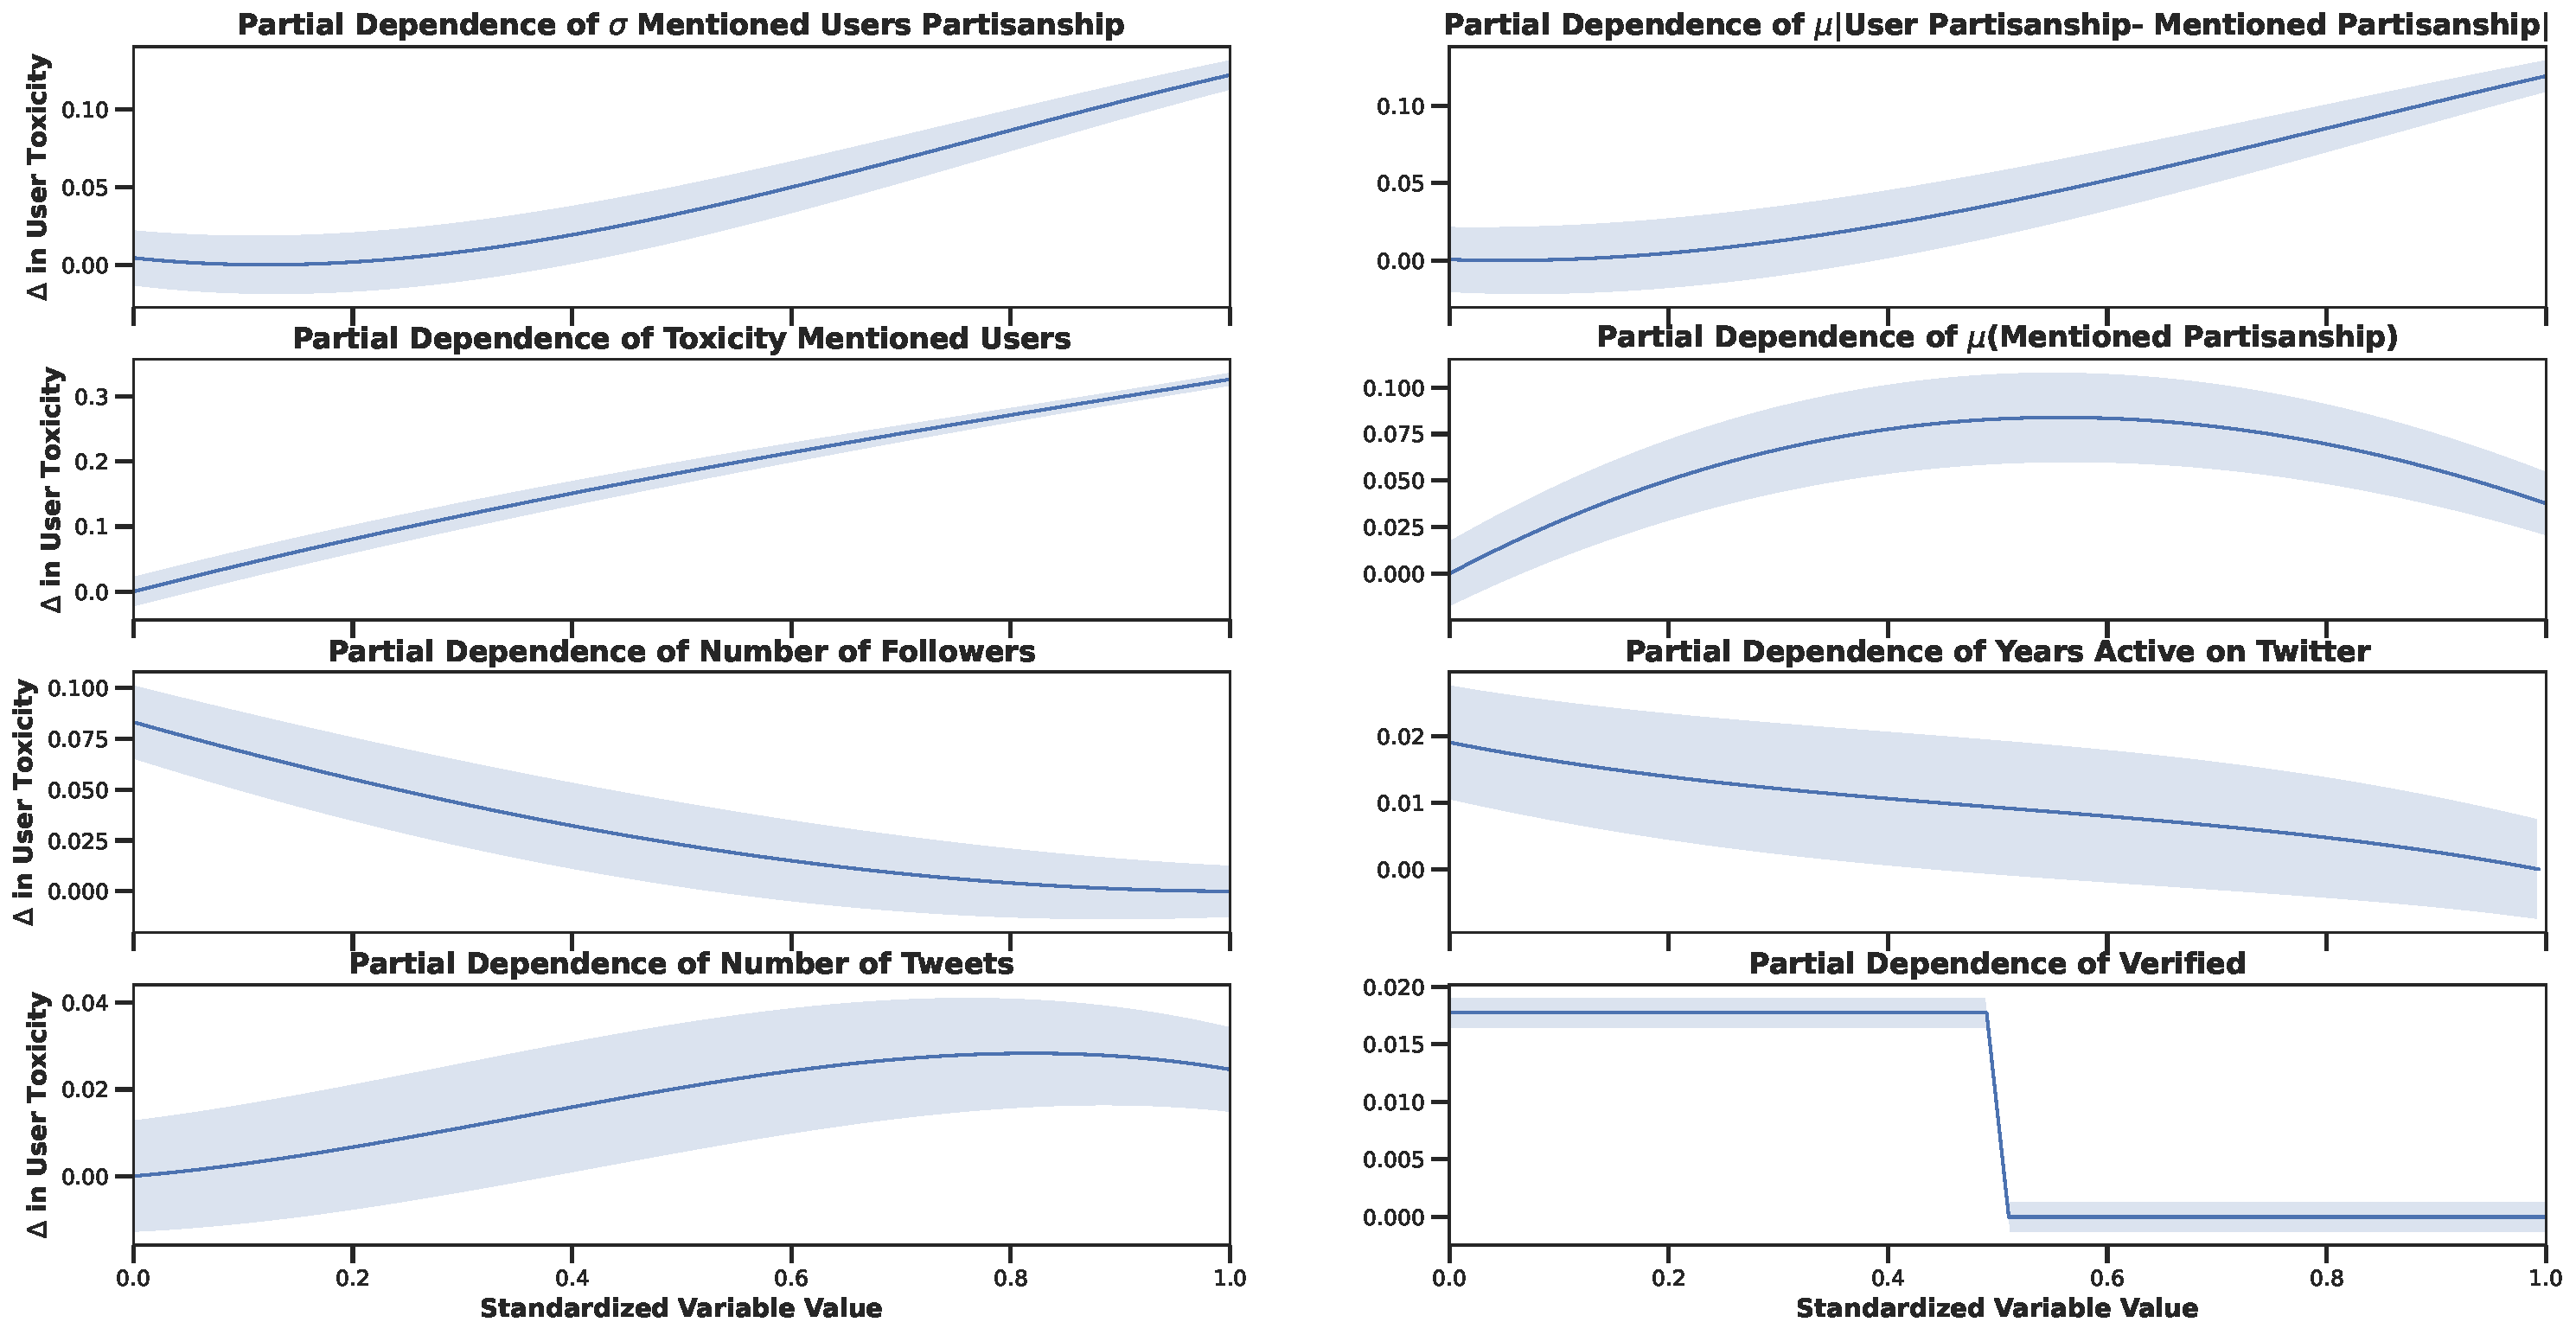
\includegraphics[width=1\columnwidth]{figures/partial_dependence_important_variables.pdf} 
\end{minipage}
\begin{minipage}[l]{1\textwidth}
\caption{Partial dependencies with 95\% Normal Confidence intervals between our fitted standardized dependent variables and user toxicity.}
\label{fig:partial-dependence-user-toxcity}
\end{minipage}

\end{figure}

\begin{table}
    \small
    \centering
    \begin{tabularx}{0.90\columnwidth}{l|rrr}
    Train $R^2$:  0.239 ,   $R^2$:  0.207  \\
    \toprule
      Dependent Variable  & Pearson Corr. $\rho$ & Kendall's $\tau$  & Permut Import. \\    \midrule
  Verified Status & ---- &-0.242 & 0.053  \\
  Years Active on Twitter & -0.197& -0.147 & 0.027 \\
  Log \# Followers & -0.206 &-0.122 & 0.205  \\
  Log \# Followed & -0.135 & -0.090 & --- \\
  Log \# Tweets in 2022 & 0.147 & 0.200  & 0.045\\
  Toxicity of Mentioned Users& 0.318& 0.362 & 0.374 \\
  partisanship  &0.054& 0.061 & --- \\
  $\sigma$(Mentioned partisanship)&0.317& 0.332	& 0.150\\
   $\mu$(Mentioned partisanship) & 0.110 &0.099 & 0.067  \\
  $\mu$|User partisanship- Mentioned partisanship|&0.287& 0.283 & 0.080\\


    
    \bottomrule
     %\multicolumn{2}{c}{ $^\ast p<0.05; \;  ^{**} p<0.01; \; ^{***}p<0.001$ }
    \end{tabularx}
  \caption{Pearson correlation $\rho$ and Kendall's $\tau$, and permutation importance of dependent variables and user's toxicity. As seen in the above table, a user's interaction with a wide political variety of users and interacting with other users with higher toxicity correlates with a given user's toxicity. } 
   \vspace{-15pt}
   \label{table:importance-user-toxicity}
\end{table}





To understand how these factors interact with and contribute to toxicity on Twitter, we fit a Generalized Additive Model (GAM) on the average toxicity score of users (Table~\ref{table:importance-user-toxicity}). When fitting our model, we perform variable selection using forward selection based on the Akaike Information Criterion~\cite{akaike2011akaike}, which ended up eliminating the number of followed accounts as well as the user partisanship as variables from our final model. Furthermore, to ensure that our model generalizes, we further reserve 10\% of our data as validation, and in our results report our model's $R^2$ value on this validation set. Finally, after fitting this regression, we further determine the estimated importance of each variable to our final model by permuting the features and seeing the estimated impact on the $R^2$ score on the validation set of our data (permutation importance is a widely used statistic for determining the relative information of features to models~\cite{altmann2010permutation}). We present the partial dependence (with 95\% Normal confidence intervals) on the user toxicity of each independent variable in Figure~\ref{fig:partial-dependence-user-toxcity} and present Pearson correlation, Kendall's $\tau$  (a more robust version of the Spearman Correlation), and each independent variable's permutation importance in Table~\ref{table:importance-user-toxicity}.  Our final model achieved a $R^2$ value of 0.239 on our training data and a $R^2$ value of 0.207 on our validation dataset, illustrating that our model does generalize to users outside of its training data.


We lastly note that to ensure the robustness of our approach, we separately perform the same analysis utilizing the toxicity scores output by the Perspective API, obtaining similar results. We present these results in Appendix~\ref{sec:perspective-user-app}.

\subsection{Baseline Account Characteristics}
We first provide an overview of how several baseline account characteristics contribute to the toxicity of each user. As seen in Table~\ref{table:importance-user-toxicity}, we do indeed observe that each of the user characteristics that we consider (to varying degrees) \emph{does} indeed have observed a correlational effect on how toxic users' tweets tend to be. We consider each of these effects below.

\vspace{2pt}\noindent
\noindent
\textbf{Verified Status.} As seen in Table~\ref{table:importance-user-toxicity} and Figure~\ref{fig:partial-dependence-user-toxcity}, as also found by Hua {et~al.}~\cite{hua2020characterizing}, whether a user is verified has a modest effect on how often they post toxic tweets, with verified users being less likely to tweet harmful or toxic messages compared to non-verified users. Overall, we find that a user's verification status has a Kendall's $\tau$ of -0.242 with their verification status and has a permutation importance of 0.053 in our final model. This suggests that when users become verified and their account is associated with their offline life, users tend to be less toxic. We note that we collected users' verification status before the implementation of Twitter Blue (users could pay 8 USD to become verified) in November 2022~\cite{Fung2023}.

\vspace{2pt}\noindent
\noindent
\textbf{Years Active on Twitter.} As users stay on Twitter, as seen in Figure~\ref{fig:partial-dependence-user-toxcity}, we observe that they are less likely to be toxic. As argued by Rajadesingan {et~al.}~\cite{rajadesingan2020quick} in their paper on Reddit, as social media users stay longer on particular platforms and adjust to interacting with other users, they tend to be less aggressive and toxic with other users. We see a similar result here, with older users being less toxic than younger ones. Overall, we observe that the number of years that a user is active on Twitter has a Pearson correlation of $\rho=-0.197$ with their average toxicity and a permutation importance of 0.027. This accords with past research that has found that news users, who are used to the social mores and norms of a given online community, may more frequently violate those norms and post toxic content~\cite{kraut2010dealing}.

\vspace{2pt}\noindent
\noindent
\textbf{Number of Followers.} Like verified status, and as argued by Marwick {et~al.}~\cite{marwick2011see}, extremely popular users are less likely overall to be toxic than users with smaller followings. These users, often create friendly public personas to interact with their followers, rarely attacking other users or posting toxic content. As seen in Figure~\ref{fig:partial-dependence-user-toxcity}, we see the same: more popular users that have more followers are less likely to post toxic tweets ($\rho=-0.206$). This variable has a permutation importance of 0.205 suggesting the high relative importance in determining the toxicity of accounts. 

%spam and fake accounts~\cite{Fishkin2022}, having an unusually small number of followers is often an indicator of a fake account. Similarly,
\vspace{2pt}\noindent
\noindent
\textbf{Number of Tweets.}
Many accounts in our Twitter dataset post several times a day, with the median account posting 614.0~times throughout 2022, and one account posting 413,658 times. As seen in Figure~\ref{fig:partial-dependence-user-toxcity} with a permutation importance of 0.045 and a Pearson correlation of $\rho=0.147$, we observe that as Twitter users post more, generally their average toxicity increases. This finding reinforces past work that suggests that accounts that post excessively and that spam Twitter, are more likely to be toxic~\cite{salehabadi2022user}. %This variable has a permutation importance of 0.045 

%Altogether, the number of tweets posted accounts for 0.75\% of the variability in user toxicity.

\begin{figure}
\begin{minipage}[l]{0.6\textwidth}
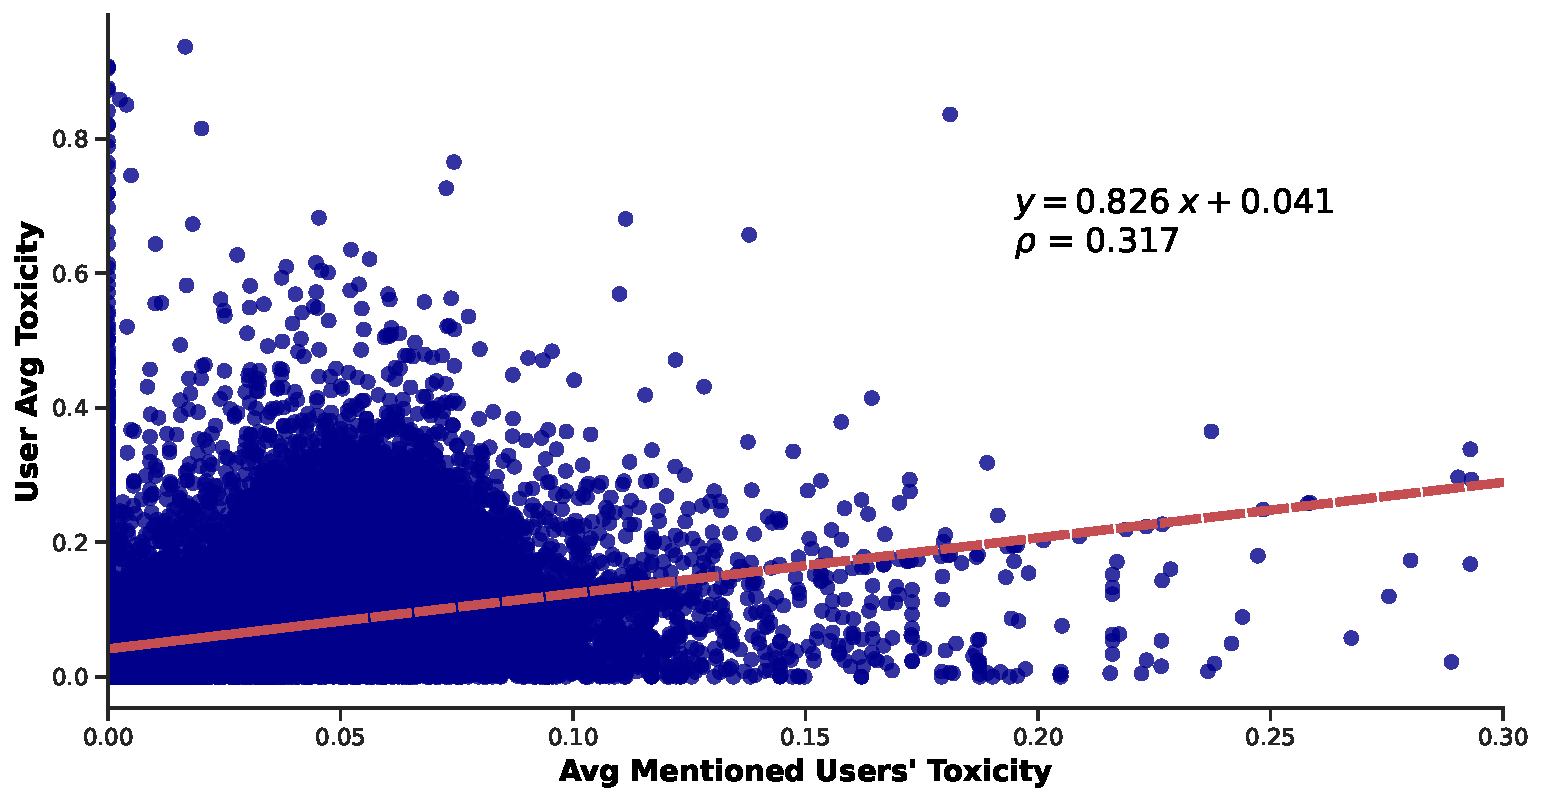
\includegraphics[width=1\columnwidth]{figures/toxicity_vs_mentioned_toxicity-20240424.pdf} 
\end{minipage}
\begin{minipage}{.33\textwidth}
  \centering
  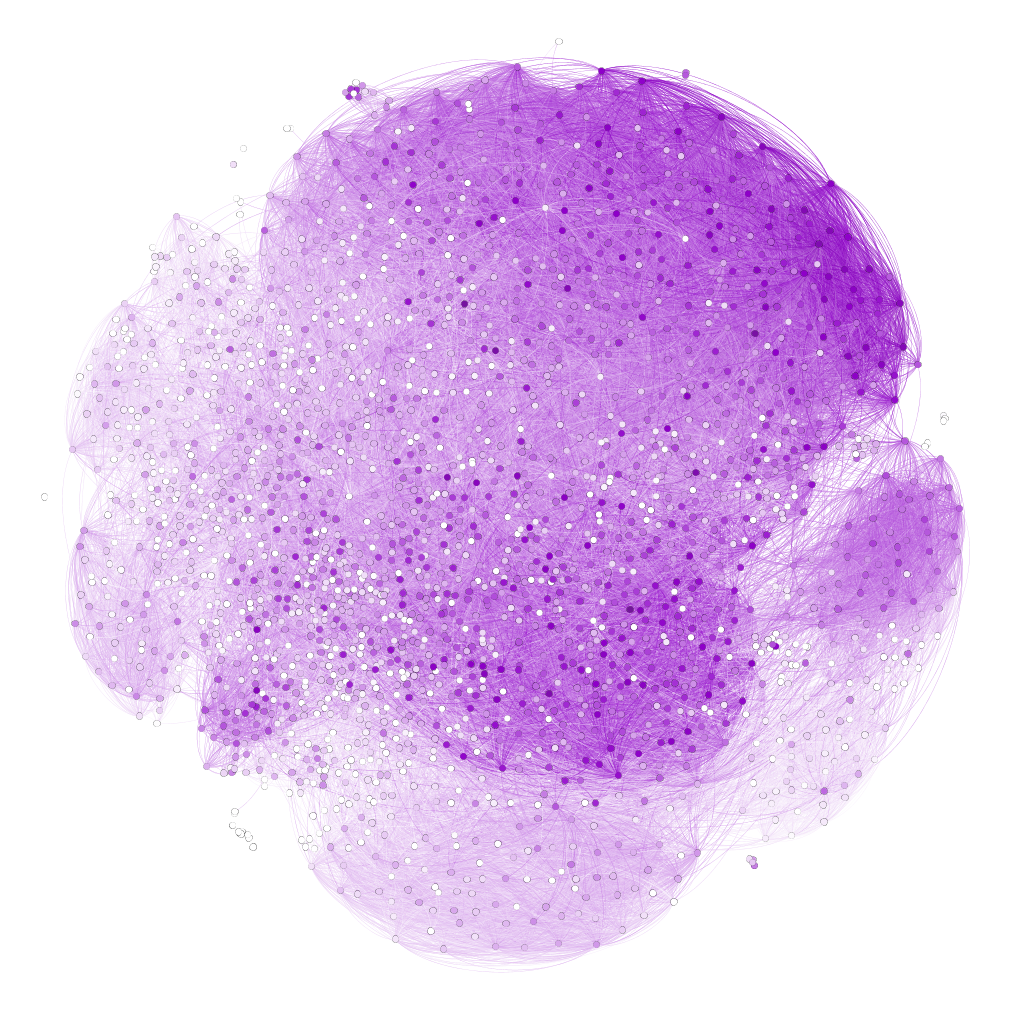
\includegraphics[width=1\linewidth]{figures/toxicity-graph.png}
  \label{fig:Twitter-reddit-toxicity-time}
\end{minipage}
\begin{minipage}[l]{1\textwidth}
\caption{The more toxic the users mentioned by a given user, on average, the more toxic the content of that particular user. Within the mention graph (the darker the purple the more toxic) of user interactions, toxicity has an assortativity coefficient of 0.071, suggesting that, to some degree, users who post toxic content have a slight tendency to mention and interact with other users who post toxic content. \label{fig:toxicity-vs-mention}}
\end{minipage}

\end{figure}

\subsection{Calculated Account Characteristics: Toxicity and Political Orientation\label{sec:calculated}}

Here we provide an overview of how the different political and toxicity measures that we calculated contribute to individual user-level toxicity. 

\vspace{2pt}\noindent
\noindent
\textbf{Toxicity of Mentioned Users.} We find that as users interact with or mention (@ing) other users who post toxic content, they themselves are more likely to be toxic. As seen in Figure~\ref{fig:partial-dependence-user-toxcity}, the average toxicity of accounts with which a user interacts has a nearly linear relationship with the user's own toxicity with very little variation. Indeed, we find this variable to be the most important in determining a user's toxicity, with it having a permutation importance of 0.374 and a Pearson correlation $\rho=0.318$. The most important of our covariates in terms of explainability, this result reinforces many prior findings about when and why particular users are toxic online~\cite{saveski2021structure,rajadesingan2020quick}. Creating a mention (@) graph among our 43,151~users and plotting users' toxicity against the toxicity of their mentioned accounts in Figure~\ref{fig:toxicity-vs-mention}, we further find some degree of assortativity based on toxicity (0.071), with more toxic users more likely to interact with each other than with non-toxic users, supporting this result. 


\begin{figure}
\begin{minipage}{.33\textwidth}
  \centering
  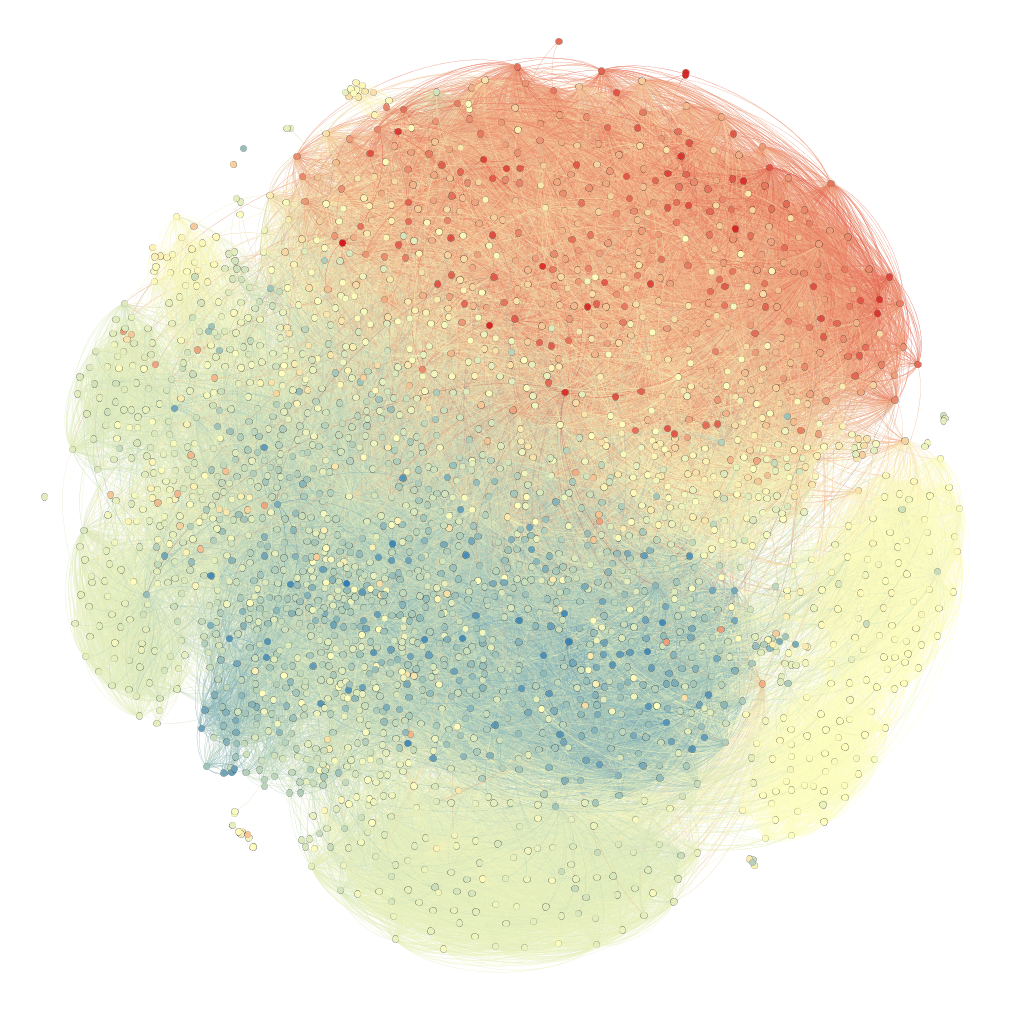
\includegraphics[width=1\linewidth]{figures/republican-democratic-graph.png}
\label{fig:twitter-reddit-partisanship-time}
\end{minipage}%
\begin{minipage}{.6\textwidth}
  \centering
  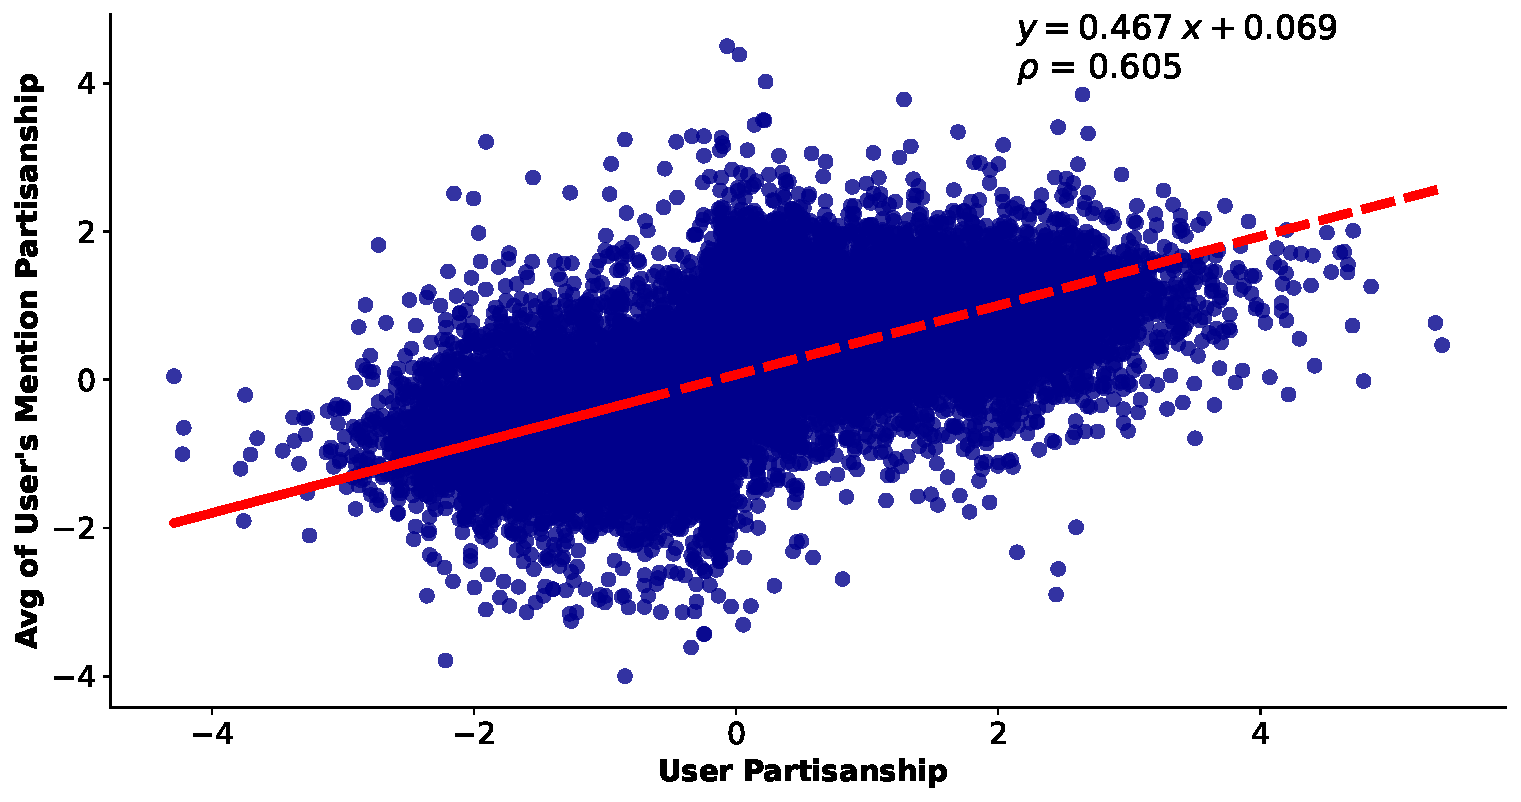
\includegraphics[width=1\linewidth]{figures/ideology_vs_avg_mention-20240429.pdf}
\label{fig:twitter-reddit-partisanship-time2}
\end{minipage}%

\begin{minipage}{1\textwidth}
\caption{Within the mention graph of user interactions (red/right-leaning and blue/left-leaning), partisanship has an assortativity coefficient of 0.266, suggesting that conservative users mention and interact more with right-leaning users while liberal users interact more with and mention other left-leaning users. Similarly, graphing the average of each user's mention's partisanship against their own partisanship, we find significant assortativity (Pearson correlation $\rho=0.605$)\label{fig:graph-of-political-interactions}
}
\end{minipage}

\end{figure}
\vspace{2pt}\noindent
\noindent
\textbf{Partisanship of Mentioned Users.} As the average value of the partisanship increases (the mentioned accounts become more right-wing), we find that the average toxicity of an account increases (Figure~\ref{fig:partial-dependence-user-toxcity}) before decreasing again on the right side of the political spectrum. We thus find that when users mention users on the political extreme, this does not indicate increased toxicity; rather we find in general that users who reference these users tend to tweet less toxic content on Twitter. This may do with the tendency that the users who reference these politically polarized/extreme users also tend to be near the political extremes themselves. Creating a mention/@  graph among our 43,151~users, we find a moderate degree of assortativity (0.266), thus finding that users, on the whole, tend to interact with other users of similar political views (Figure~\ref{fig:graph-of-political-interactions}) and that this tendency is not necessarily correlated with increased toxicity.  Graphing the average partisanship of a user's mention against their own partisanship we further observe a high assortativity (Pearson correlation of $\rho=0.605$). 
\begin{figure}
\begin{minipage}[l]{0.48\textwidth}
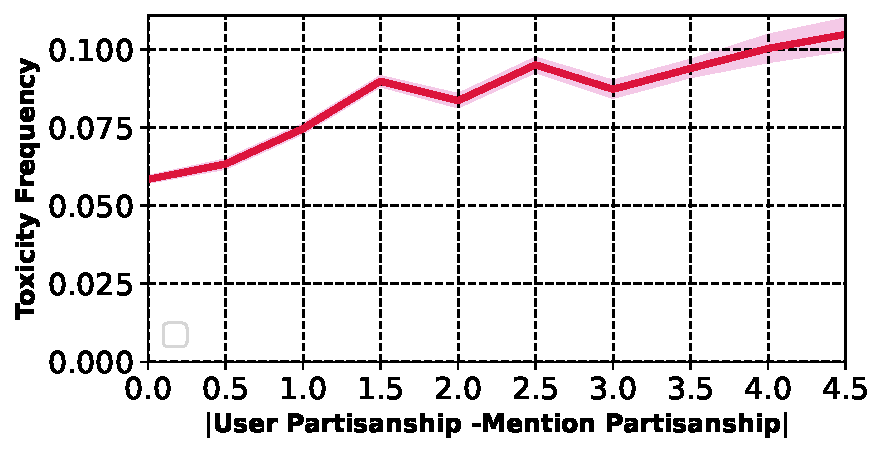
\includegraphics[width=1\columnwidth]{figures/toxicity_vs_mention-20240428.pdf}
\end{minipage}
\begin{minipage}[l]{0.33\textwidth}
\caption{As the difference in the partisanship of users and those that they mention/@ increases, the probability of users tweeting toxicly increases. 95\% Normal Confidence Intervals.
\label{fig:toxicity_vs_mention-new}}
\end{minipage}
\end{figure}

Instead, as was seen in (Figure~\ref{fig:partial-dependence-user-toxcity}) it is the difference in partisanship between a user and their mentions that linearly determines the toxicity of users. The average difference in the partisanship between a user and their mentioned accounts has a $\rho = 0.287$ Pearson correlation with the user's own toxicity and has a permutation importance of 0.080. Indeed, as seen in Figure~\ref{fig:toxicity_vs_mention-new}, we observe across our entire dataset that as the difference between a user's partisanship and the partisanship of the corresponding user that mention/@ increases the probability that they tweet toxicly increases. This illustrates, as found elsewhere~\cite{hanley2023sub,mamakos2023social}, that as users interact with more users different in partisanship than themselves, they are more likely to be toxic.  As an example a left-wing user (-1.53) with a particularly high standard deviation for the diversity of their mentions (1.818), often engaging in heated discussion with right-wing and left-wing accounts wrote the tweet concerning the former Republican US president Donald Trump:
\begin{displayquote}
\small
\textit{
This is so indescribably fucked up. Except I love Nancy Pelosi giving him the shiv.}
\end{displayquote}
\noindent
Similarly, a different  left-wing account (-1.504), which also regularly interacts with right-wing and left-wing accounts (1.65), regarding former Republican US president Donald Trump's son wrote:
\begin{displayquote}
\small
\textit{
Fuck him. No, seriously, fuck him. If anyone’s a welfare queen it’s him...}
\end{displayquote}
\noindent


\begin{figure}
\begin{minipage}[l]{0.48\textwidth}
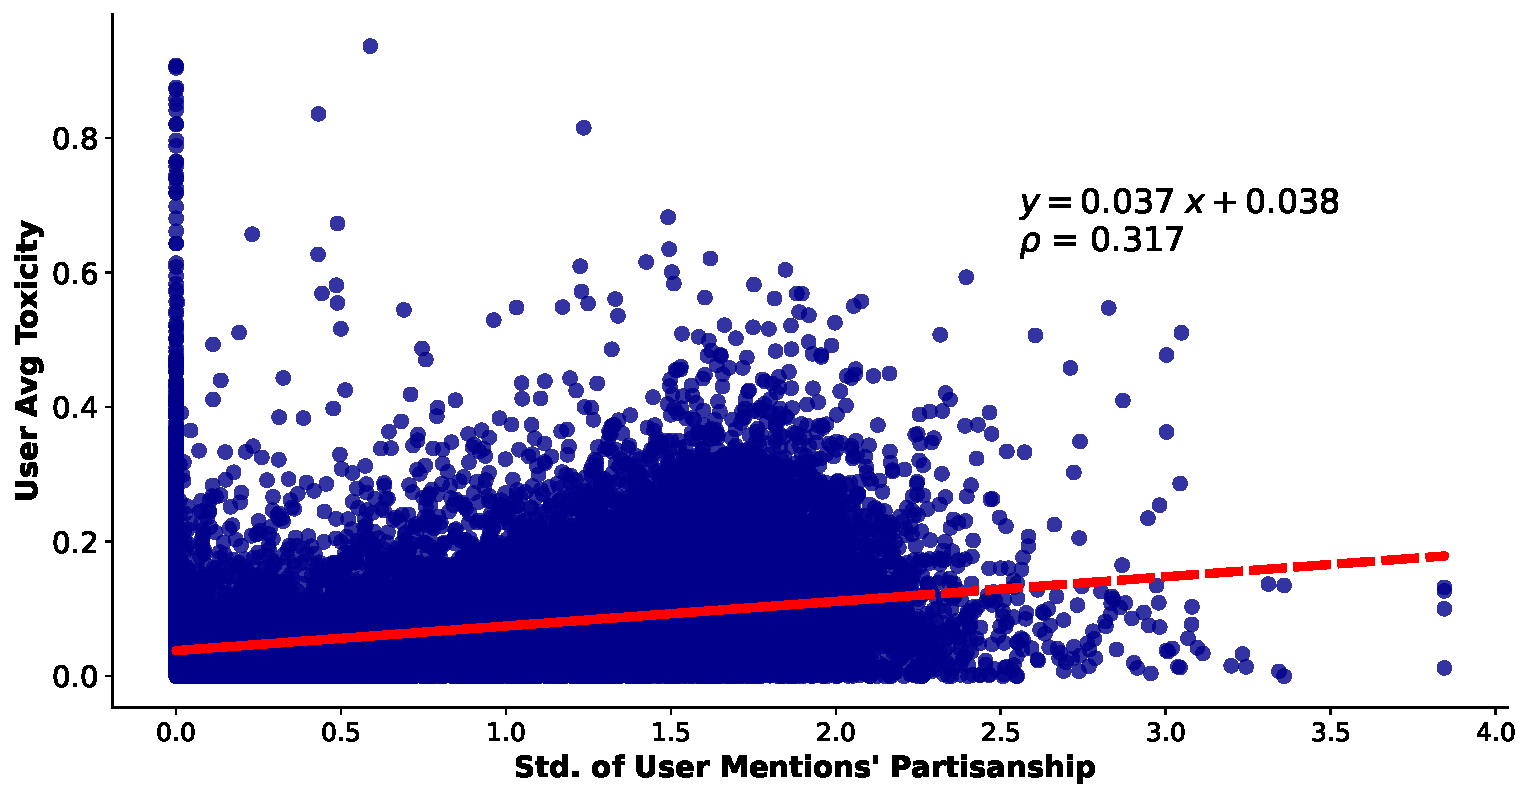
\includegraphics[width=1\columnwidth]{figures/toxicity_vs_avg_mention-20240429.pdf}
\end{minipage}
\begin{minipage}[l]{0.33\textwidth}
\caption{As users mention a wider range of users along the political spectrum they are more likely to tweet toxic messages. 
\label{fig:politican-variance-toxicity2}}
\end{minipage}
\end{figure}


\vspace{2pt}\noindent
\noindent
\textbf{The Political Diversity of Mentions.}
In addition to finding that as users interact with more users different than themselves, from Figure~\ref{fig:partial-dependence-user-toxcity} and Table~\ref{table:importance-user-toxicity}, we find that as users mention/@ a wider political diversity of users, the more toxic their own tweets. With a Pearson correlation of $\rho =0.317$ and a permutation importance of  0.15, we see that this feature is relatively important in our fit model with it heavily contributing to the prediction of a user's toxicity (Figure~\ref{fig:politican-variance-toxicity2}).  This reinforces the finding of Mamakos et~al.~\cite{mamakos2023social}. who also found that when users engage with both left-leaning and right-leaning accounts on Reddit, they are more likely to engage in toxic behaviors on the platform. 


%We thus see these accounts which often engage with a wide diversity and with users that are different from themselves, often tweet toxically sometimes concerning their political opponents.  







\subsection{Summary}
In this section, using a GAM, we explored the role that several user-level characteristics have on the rate of user toxicity on Twitter. We find, most importantly, that users who interact and mention other users who regularly post toxic content are more likely to be toxic themselves. Similarly, we found the more a given user interacts with a politically diverse set of accounts, the more likely that account is to tweet toxic content. We replicate these results with the Perspective API in Appendix~\ref{sec:perspective-user-app} getting similar results. 
